\paragraph*{Характеристические функции вероятностных мер, случайных величин и векторов}

\begin{definition} Пусть $\xi$ - случайный вектор $\in \R^k$, тогда $$\charac{\xi}{x} = \E e^{i<\xi, x>} = \E (cos<\xi, x> + i<\xi, x>) = \E cos<\xi, x> + i \E sin<\xi, x>$$, $\charac{\xi}{x}: \R^k \to \C$ - характеристическая функция $\xi$, где $<x, y>$ -- скалярное произведение. \end{definition}

\paragraph*{Примеры}
\begin{enumerate}
    \item $\xi \sim Bern(p)$, тогда $\charac{\xi}{x} = pe^{ix} + (1 - p)$
    \item 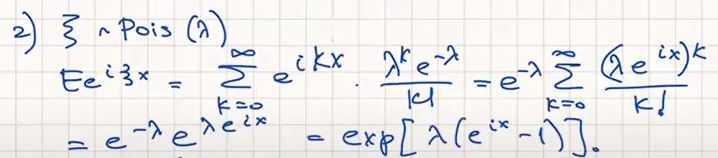
\includegraphics[]{images/pt1.JPG}
    \item $\xi \sim U[a, b]$, тогда $\charac{\xi}{x} = \E e^{ix\xi} = \frac{1}{b - a}\int\limits_a^b e^{ixt}dt = \frac{e^{itb} - e^{ita}}{it(b - a)}$
    \item $\xi \sim \mathcal{N}(0, 1)$, тогда $\charac{\xi}{x} = \int\limits_\R \frac{1}{\sqrt{2\pi}} e^{itx - \frac{t^2}{2}} dt = \int\limits_\R \frac{1}{\sqrt{2\pi}} e^{-\frac{(t - ix)^2}{2} - \frac{x^2}{2}} dt = e^{-\frac{x^2}{2}}$
    \item $\xi \sim \mathcal{N}(a, \sigma^2) \Longrightarrow \frac{\xi - a}{\sigma} \sim \mathcal{N}(0, 1)$
    $$
    \charac{\frac{\xi - a}{\sigma}}{x} = \E e^{i\frac{\xi - a}{\sigma}x} = e^{-\frac{x^2}{2}} \Longrightarrow \charac{\frac{\xi}{\sigma}}{x} =e^{ia\frac{x}{\sigma} - \frac{x^2}{2}} \Longrightarrow \charac{\xi}{x} = \charac{\frac{\xi}{\sigma}}{\sigma x} = e^{iax - \frac{\sigma^2x^2}{2}}
    $$
\end{enumerate}

\begin{theorem}[О единственности]

Если $\charac{\xi}{x}, \charac{\eta}{x}$ - характеристические функции случайных векторов одинаковой размерности и $\forall x \in \R^n \ \charac{\xi}{x} = \charac{\eta}{x}$, то $\xi = \eta$ по распределению (то есть случайные векторы имеют одинаковое распределение)

\end{theorem}

\begin{theorem}[О независимости]

$\xi_1, \ldots, \xi_n$ независимы $\Longleftrightarrow$ $\charac{(\xi_1, \ldots, \xi_n)}{x_1, \ldots, x_n} = \prod\limits_{j = 1}^n \charac{\xi_j}{x_j}$

\end{theorem}

\begin{proof} 
$\Longrightarrow$ 
$\xi_1, \ldots, \xi_n$ независимы, а значит и $(\cos(\xi_1x_1), \sin(\xi_1x_1)), \ldots, (\cos(\xi_nx_n), \sin(\xi_nx_n)))$ независимы. Тогда
\begin{multline*}
    \charac{(\xi_1, \ldots, \xi_n)}{x_1, \ldots, x_n} = \E e^{i(x_1\xi_1 + \ldots + x_x\xi_n)} = \E\brackets{\prod\limits_{j = 1}^n (\cos(\xi_jx_j) + i\sin(\xi_jx_j))} = \\
    = \prod\limits_{j = 1}^n\E\brackets{ \cos(\xi_jx_j) + i\sin(\xi_jx_j)} = \prod\limits_{j = 1}^n \E e^{ix_j\xi_j} = \prod\limits_{j = 1}^n \charac{\xi_j}{x_j}
\end{multline*}

$\Longleftarrow$
Рассмотрим $\eta = (\eta_1, \ldots, \eta_n)$ такие, что компоненты вектора независимы и $\forall j \leqslant n \ \xi_j = \eta_j$ по распределению.

Тогда $\charac{\eta}{x_1, \ldots, x_n} = \prod\limits_{j = 1}^n \charac{\eta_j}{x_j} = \prod\limits_{j = 1}^n \charac{\xi_j}{x_j} = \charac{(\xi_1, \ldots, \xi_n)}{x_1, \ldots, x_n}$. Значит по теореме о единственности $\eta = (\xi_1, \ldots, \xi_n)$ по распределению, а значит $\xi_1, \ldots, \xi_n$ независимы в совокупности. Вопрос: почему существует такое $\eta$\end{proof}

\paragraph*{Свертка}
\begin{statement}
$\eta, \xi$ независимы $\implies \varphi_{\xi + \eta}(x) = \varphi_{\xi}(x)\varphi_{\eta}(x)$
\end{statement}

\begin{proof} $\varphi_{\xi + \eta}(x) = \E e^{i(\xi + \eta)x} = \E e^{i\xi x} e^{i \eta x}= \E e^{i\xi x} \E e^{i \eta x} = \varphi_{\xi}(x)\varphi_{\eta}(x)$ \end{proof}
\bigskip

\begin{statement}
$\implies \varphi_{a\xi + b}(x) = e^{ibx} \varphi_{\xi}(ax)$
\end{statement}

\begin{proof} $\varphi_{a\xi + b}(x) = \E e^{i(a\xi + b)x} = \E e^{ia\xi x} e^{i bx}= e^{i bx} \E e^{i\xi ax} = e^{ibx} \varphi_{\xi}(ax)$ \end{proof}